\chapter{Traitement des données et classification}
Comme décidé lors de l'analyse de l'état de l'art et les réflexions de départ, la première analyse qui est faite, est de faire de la classification avant de tester les résultats de la régression. 

L'algorithme qui a été sélectionné pour effectuer cette tâche est SVM (Support Vector Machines). Ce chapitre va décrire les différentes étapes qui ont été réalisées pour traiter les données et utiliser l'algorithme.

La programmation a été réalisée sur l'environnement PyCharm PROFESSIONAL 2018.2 et dans le langage Python. Cet environnement m'est le plus familier, car il est étudié dans différents cours, c'est pourquoi mon choix s'est porté sur ce dernier. 

%\begin{figure}[htp]
% \begin{center}
%  
\includegraphics[scale=0.6]{figures/pycharm.png}
%  \caption{Logiciel utilisé pour le développement}
%  \label{fig:pycharm} %% NOTE: always label *after* caption!
% \end{center}
%\end{figure}

\section{Structure du traitement}
Pour le traitement de données pour un apprentissage à l'aide d'un algorithme il est conseillé d'avoir différentes étapes voir Figure \ref{fig:process}. 

\begin{enumerate} 
 \item Acquisition des données : Étape délicate et très importante dans ce projet.
 \item Prétraitement: Étape de traitement sur les données brutes se trouvant dans le jeu de données.
 \item Extraction des caractéristiques : Étape qui consiste à extraire les caractéristiques qui seront utilisées par l’algorithme pour faire la reconnaissance. 
 \item Reconnaissance : Utilisation d’un algorithme pour effectuer la reconnaissance des positions. 
 \item Décision :  Cette étape consiste, si cela est nécessaire, à décider du résultat final à l’aide d’une fusion, cela n'a pas été utilisé.
\end{enumerate}

\begin{figure}[H]
 \begin{center}
  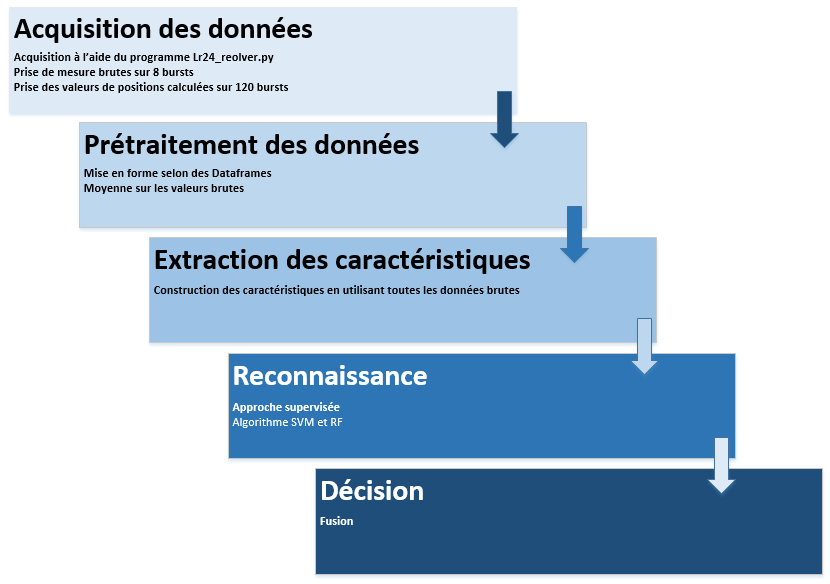
\includegraphics[scale=0.6]{figures/processing.png}
  \caption{Flux de traitement de l'information}
  \label{fig:process} %% NOTE: always label *after* caption!
 \end{center}
\end{figure}

Le premier point est l'acquisition de données qui est décrit au chapitre précédent. C'est une étape primordiale, car c'est grâce à ces données que toute la suite de l'analyse va dépendre. Dans le cadre de ce projet, on remarque vite que si les données ne sont pas prises de manière rigoureuse, cela ne fonctionne pas.

Le prétraitement consiste à utiliser les données disponibles et de les exploiter. Dans un premier temps, les données sont lues depuis un fichier *.npy qui représente des données NumPy. NumPy est une extension du langage de programmation Python, destinée à manipuler des matrices ou tableaux multidimensionnels ainsi que des fonctions mathématiques opérant sur ces tableaux. Plus précisément, cette bibliothèque logicielle libre (open source) fournit de multiples fonctions permettant notamment de créer directement un tableau depuis un fichier ou au contraire de sauvegarder un tableau dans un fichier, et manipuler des vecteurs, matrices et polynômes \cite{WIKI2}. 

Depuis ce fichier, plusieurs traitements sont effectués afin de transformer les données et les mettre dans un format permettant un traitement simple, le format "Dataframe" a été choisi et appartient à la librairie Pandas. Pandas est une bibliothèque écrite pour le langage de programmation Python permettant la manipulation et l'analyse des données. Elle propose en particulier des structures de données et des opérations de manipulation de tableaux numériques et de séries temporelles \cite{WIKI3}. À partir de là, il est possible d'utiliser les données afin d'en extraire des caractéristiques qui est l'étape suivante. Ce point sera détaillé plus loin afin de mieux comprendre ce qui a été utilisé pour que l'algorithme puisse au mieux reconnaitre les différentes positions. 

L'étape de reconnaissance consiste à entrainer un système avec les caractéristiques sélectionnées à partir des données et ensuite de valider que notre algorithme est capable de reconnaitre de nouvelles mesures. Ce point est également détaillé plus bas. 

Finalement, dans ce type d'analyse, il existe souvent une partie décision. Cela peut se faire, car deux algorithmes différents sont utilisés et il est nécessaire de décider quel est le meilleur résultat. Dans le cadre de ce projet, il n'a pas été nécessaire d'utiliser cela, car il n'a pas été possible dans le temps imparti de tester plusieurs techniques et donc la fusion n'était pas utile.

\section{Extraction des caractéristiques}
Ce chapitre traite des caractéristiques qui seront utilisées par l'algorithme afin de déterminer à quelle classe elles appartiennent. La Figue \ref{fig:dataframe} montre comment se présentent les données. Il est possible de les séparer et d'isoler chaque mesure. Chaque mesure est composée des données pour les quarante canaux (colonne : Canal). Les mesures qui peuvent être exploitées pour effectuer la classification sont les mesures brutes de différence de distance (Sx.x). Il serait aussi possible d'exploiter la position fournie par le programme de prise de mesures, mais cette dernière n'est pas assez représentative. C'est pour cette raison que deux types de classification ont été effectués. 

La première consiste à utiliser les données brutes et de travailler avec ces dernières pour extraire d'autres caractéristiques. Les principales qui ont été testées sont décrites ci-dessous.

\begin{enumerate}
 \item Toutes les données (raw) : Cela consiste à prendre toutes les mesures brutes de tous les canaux et de les mettre les unes après les autres. Ce qui veut dire 320 valeurs (quarante canaux fois 2x chaque esclave).
 \item Un canal (raw) : Cette façon de faire est identique à la précédente sauf qu'un seul canal est pris en compte ce qui fait 8 valeurs (un canal fois 2x chaque esclave).
 \item Moyenne : La moyenne est faite sur les quarante canaux par esclave ce qui va donner huit caractéristiques supplémentaires.
 \item Variance : La variance est une mesure qui permet de caractériser la dispersion d'un échantillon. Elle est utilisée pour voir la dispersion des valeurs par esclave sur les quarante canaux. 
 \item Déviation standard : La déviation standard équivaut à la racine carrée de la variance. C'est donc une mesure de dispersion qui est faite également par esclave sur les quarante canaux. 
 \item Quantile : Un quantile correspond à séparer les données en partie de taille égale. C'est-à-dire que chaque partie doit contenir le même nombre de données. Cela est également utilisé pour séparer les données au niveau des canaux pour un esclave.
 \item Médiane : La médiane est en quelque sorte le quantile qui sépare des données en deux parties de même taille. 
 \item covariance : La covariance permet de voir la corrélation entre des variables. Cette mesure est effectuée par esclave sur tous les canaux.  
\end{enumerate}
 
La deuxième consiste à utiliser uniquement la position fournie par le programme de prise de mesure. Cette position est mémorisée après avoir convergée et ce qui fait que les caractéristiques disponibles sont la coordonnée X et la coordonnée Y. Comme il n'y a que deux caractéristiques, il sera difficile d'effectuer différents traitements sur ces données si l'algorithme n'arrive pas différencier les classes. 

Les résultats de ces deux différentes approches seront détaillés au chapitre suivant. 

\begin{figure}[H]
 \begin{center}
  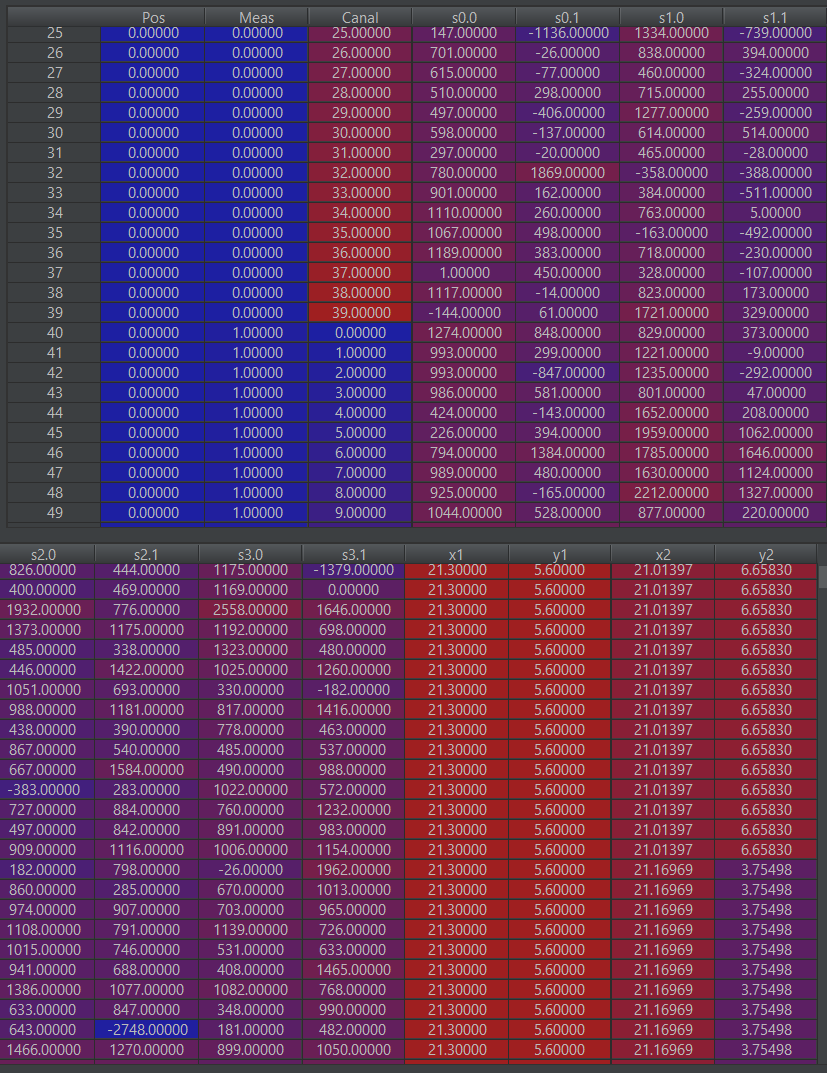
\includegraphics[scale=0.6]{figures/dataframe2.png}
  \caption{Données sous forme de dataframe pour le traitement et l'extraction des caractéristiques}
  \label{fig:dataframe} %% NOTE: always label *after* caption!
 \end{center}
\end{figure}

\section{Reconnaissance - Algorithme}
Le choix de l'algorithme a été fait par rapport à l'état de l'art qui a été effectué en début de projet. Comme déjà mentionné, l'algorithme qui a été retenu est SVM (Support Vector Machine). Cette solution permet de laisser le projet évoluer en utilisant dans un premier temps la solution pour la classification et ensuite en utilisant SVM pour la régression. 

Support Vector Machine est un algorithme supervisé qui permet de faire de la classification en essayant de trouver le meilleur hyperplan. La librairie scikit learn a été utilisée et je me suis servie de sklearn.svm.SVC (System Vector Classification).

L’implémentation de l’algorithme est facile une fois que les labels et les caractéristiques ont été extraits. Dans un premier temps, le canevas de base a été mis en place en utilisant les données brutes des mesures de "ranging". Cela a permis de faire les premiers réglages. 

Afin d'entrainer et de tester l'efficacité de l'algorithme, il est nécessaire de partager les données en trois jeux. Il y a un jeu qui est utilisé pour l'entrainement, un jeu qui est utilisé pour valider l'entrainement qui vient d'être réalisé et un troisième jeu qui sert uniquement pour le résultat final. Dans ce dernier jeu, ce sont des données que l'algorithme n'a jamais vues. La Figure \ref{fig:datasep} permet d'illustrer cette séparation. IL est également possible de voir que les données d'entrainement et de validation vont de pair. Pour ma part, j'ai décidé d'effectuer une cross-validation. C'est-à-dire qu'à chaque lancement le partage des données n'est jamais identique. La seule chose qui est respectée est qu'il y aura toujours 20\% de données pour la validation et 80\% pour l'entrainement. Une autre chose qui est à vérifier c'est que les jeux de données soient balancés. Cela veut dire qu'il doit y avoir le même nombre de données de chaque classe dans chaque jeu. Cela donnerait de mauvais résultats si l'entrainement est fait avec les classes 1,2,et 3 et que la validation se fait avec des données des classes 4 et 5 par exemple. 

\begin{figure}[htp]
 \begin{center}
  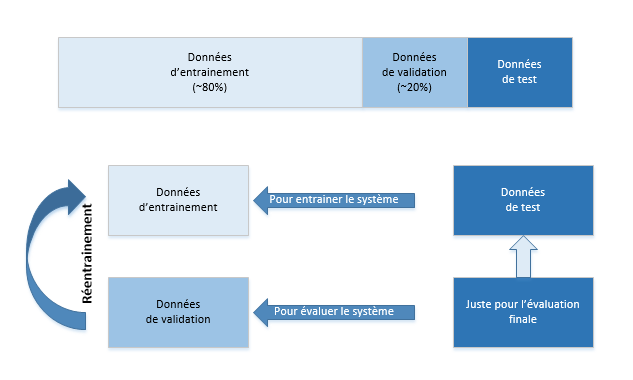
\includegraphics[scale=0.7]{figures/data_separation.png}
  \caption{Partage des données}
  \label{fig:datasep} %% NOTE: always label *after* caption!
 \end{center}
\end{figure}

\subsection{Hyper paramètres}
L'algorithme SVM utilise plusieurs paramètres qu'il a été nécessaire de chercher pour obtenir les meilleurs. Seuls le Kernel, le paramètre C et le paramètre gamma ont été cherchés. Une forte valeur de C tente de minimiser les erreurs de classification des données d'entraînement et une faible valeur essaie de maintenir une classification lisse. Concernant le gamma, plus il est grand , plus la cloche de la gaussienne est étroite voir Figure \ref{fig:c_gamma}. 

\begin{figure}[htp]
 \begin{center}
  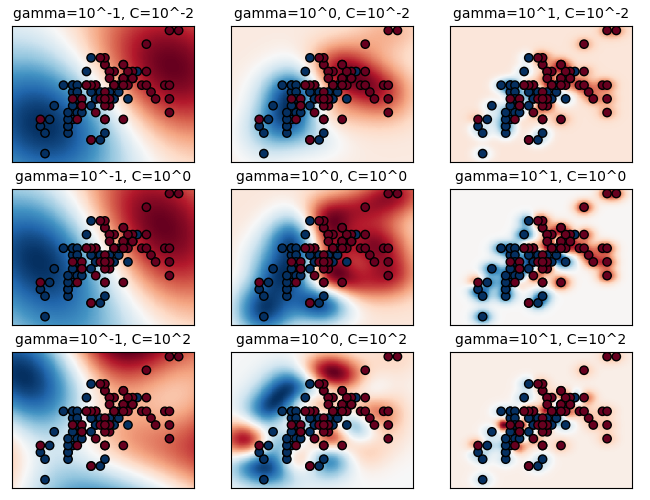
\includegraphics[scale=0.7]{figures/c_gamma_param.png}
  \caption{Influence des paramètres C et gamma}
  \label{fig:c_gamma} %% NOTE: always label *after* caption!
 \end{center}
\end{figure}

La première chose qui a été faite a été de trouver le meilleur Kernel pour cette classification. Les Kernel suivants ont été testés : linear, rbf, poly, sigmoid. Celui qui a donné les meilleurs résultats et le Kernel linear.

Suite à cela, un grid-search est effectué sur les paramètres C et gamma. Les meilleurs résultats obtenus sont avec un C égal à 1 et un gamma égal à 0.001. 

\section{Validation et résultats}
Cette section va présenter l'évolution des résultats obtenus au cours du développement. Voici un résumé des données acquises selon la Figure \ref{fig:mesures} : 

\begin{enumerate}
 \item Mesures de "ranging" effectuées sur les points Sx qui correspondent aux points que l'on souhaite retrouver (40x sur chaque point).
 \item Mesures de "ranging" effectuées sur les points Sx à un moment différent que les quarante mesures précédentes (5x sur chaque point).
 \item Mesures de "ranging" effectuées sur les points Tx. Ces points sont pris afin de voir si le plus proche voisin est retrouvé.
 \item Mesures de position effectuées sur les points Sx (40x + 5x sur chaque point).
 \item Mesures de position effectuées sur les points Tx (5x sur chaque point) 
\end{enumerate}

Ces différentes prises de données permettent de faire plusieurs analyses et comprendre de façon plus claire comment le système se comporte.

Les résultats sont évalués à l'aide des matrices de confusion, mais également à l'aide de la mesure de précision, du F1-Score macro et finalement du F1-Score micro. 

La Figure \ref{fig:precisonrecall} montre ce que représente la précision et le rappel. Ces deux notions sont utilisées pour calculer le F1-Score de la manière suivante :

F1\_score = 2((Précision * rappel)/(Précision + rappel))

Le micro ou macro-avarage sont utilisés pour analyser les données de manière différente. Pour le calcul du macro-avarage, il faut additionner les précisions de chaque classe et les diviser par le nombre de classes. Dans ce cas, il se pourrait qu'une classe soit très mauvaise et déséquilibrée, mais que les autres remontent le score. Si maintenant on parle du micro-avarage, le calcul se fait en additionnant les vrais positifs et en les divisant par le nombre total de points. Cette manière de faire va donner un score plus bas si une classe est déséquilibrée \cite{DATASCI}. 

Dans le cadre de cette analyse, toutes les classes possèdent le même nombre de données.

\begin{figure}[htp]
 \begin{center}
  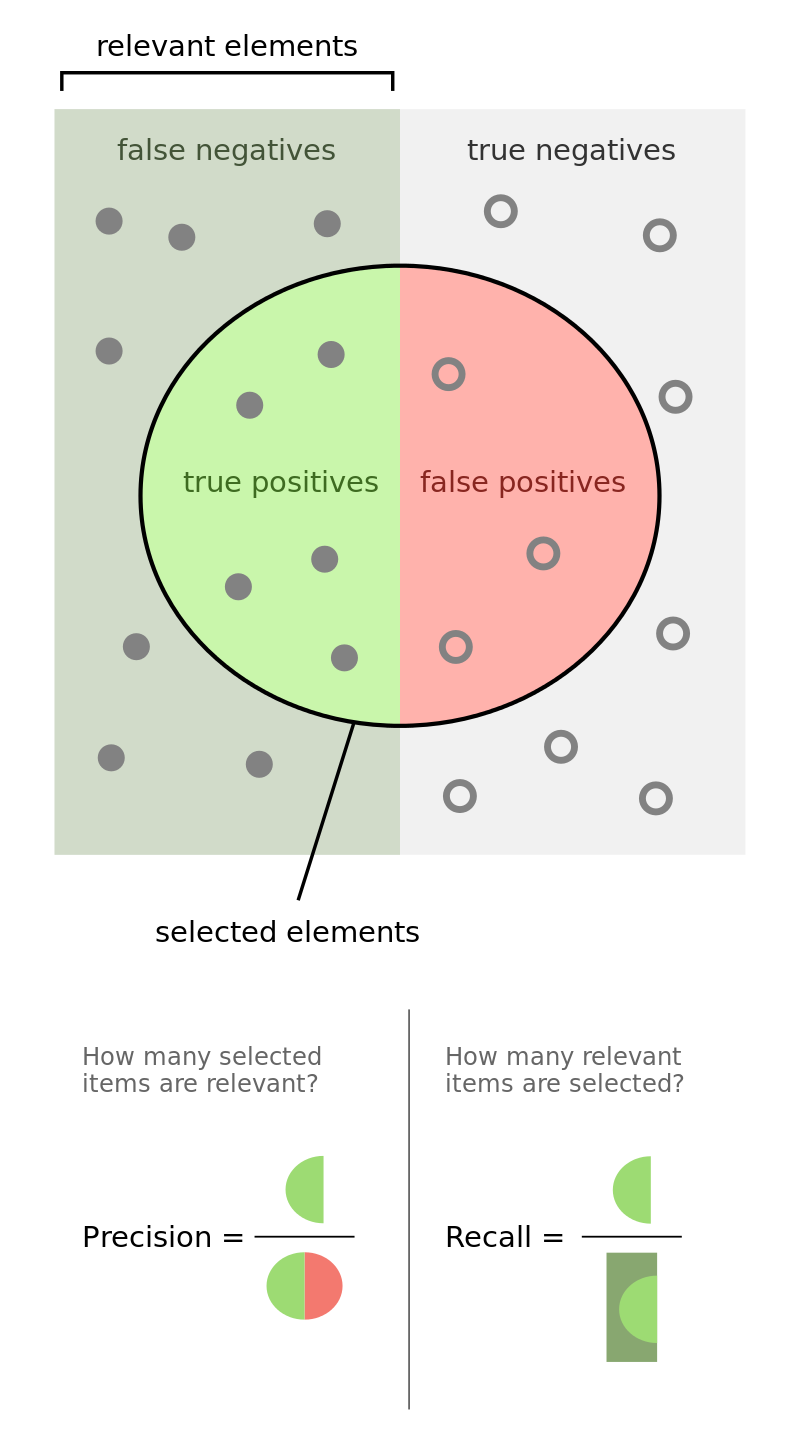
\includegraphics[scale=0.3]{figures/precisionrecall.png}
  \caption{Représentation de la précision et du rappel \cite{WIKI}}
  \label{fig:precisonrecall} %% NOTE: always label *after* caption!
 \end{center}
\end{figure}

\subsection{Résultats en utilisant les données de "ranging"}
Ce chapitre va présenter les résultats qui ont été obtenus à partir des données brutes de "ranging" fournies par le programme de mesures. Plusieurs traitements sont faits sur ces mesures afin d'améliorer les résultats. Le calcul de position est également disponible, mais n'est pas très représentatif, car calculé uniquement à partir de huit valeurs de ranging (deux sur chaque esclave).

Afin d'avoir une meilleure vue de ce que représentent les positions calculées sur peu d'échantillons, la Figure \ref{fig:plotPos} montre le positionnement de ces points calculés par rapport à la position réelle de l'espion. Les gros points de couleurs représentent la position réelle et les petits points de couleurs représentent les positions calculées. La croix noire représente la position du master. On remarque que les petits points sont bien plus espacés que lorsqu’on laisse converger la position (Figrure \ref{fig:plotPosConv}), mais il y a tout de même une séparation entre les ensembles.

\begin{figure}[htp]
 \begin{center}
  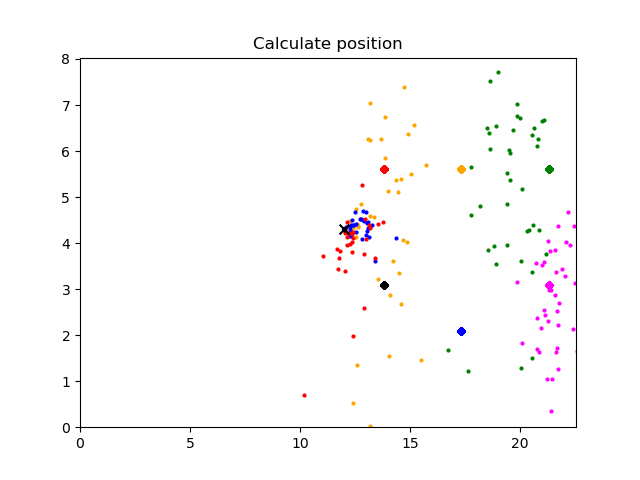
\includegraphics[scale=0.8]{figures/plot_pos.PNG}
  \caption{Représentation des points non convergé par rapport aux positions réelles}
  \label{fig:plotPos} %% NOTE: always label *after* caption!
 \end{center}
\end{figure}

La Figure \ref{fig:plotPos} met en évidence un phénomène qui tend à faire rapprocher les points sur la position du maitre. Cet effet qui se trouve dans le laboratoire où les mesures ont été effectuées complique la reconnaissance de position.

Ci-dessous, une énumération des couleurs et de la position associée : 
\begin{enumerate}
 \item Couleur verte (SO) : x = 21.30m / y = 5.60m
 \item Couleur jaune (S1)  : x = 17.30m / y = 5.60m
 \item Couleur bleue (S2) : x = 17.30m / y = 2.10m
 \item Couleur rose (S3) : x = 21.30m / y = 3.10m
 \item Couleur rouge (S4) : x = 13.80m / y = 5.60m 
 \item Couleur noire (S5) : x = 13.80m / y = 3.10m 
\end{enumerate} 

Comme décrit plus haut, toute une série de tests ont été effectués afin de trouver d'une part les meilleurs paramètres et d'autre part de trouver les caractéristiques les plus probantes. Dans tous les essais réalisés, seuls, trois seront détaillés ci-dessous: Résultats obtenus en utilisant uniquement les données de "ranging", résultats obtenus en utilisant uniquement les données de position et finalement présentation de la solution retenue qui utilise la médiane, les données "ranging", les quantiles et la variance.

\subsubsection{Résultat en utilisant toutes les données de ranging brutes}
Le premier test qui a été effectué a été de prendre toutes les données brutes des valeurs de ranging. Cela consiste à prendre chacune des mesures des quatre esclaves sur les quarante canaux et de les mettre les unes à côté des autres pour en créer une caractéristique. Cela est effectué pour chacune des mesures (quarante par position).  

La Figure \ref{fig:matPosSxTRaw} présente le résultat obtenu lorsque l'entrainement est fait avec 32 des 40 mesures sur une même position et testé avec les huit restants. Le résultat obtenu est impressionnant et offre une précision entre 95\% et 100\%. Les positions sont très bien reconnues. La variation de pourcentage pour la reconnaissance vient du fait qu'à chaque lancement, le programme exclut huit autres mesures.

La matrice de confusion représentée est donnée avec des mesures qui ont été faites sur un même point sans bouger l'espion. Le F1-score macro est de 0.9791 et un F1-score micro de 0.9792.  

%Accuracy with optimisation 97.91666666666666 %
%Accuracy 0.9791666666666666
%F1-Score macro : 0.9790849673202615
%F1-Score micro: 0.9791666666666666
\begin{figure}[htp]
 \begin{center}
  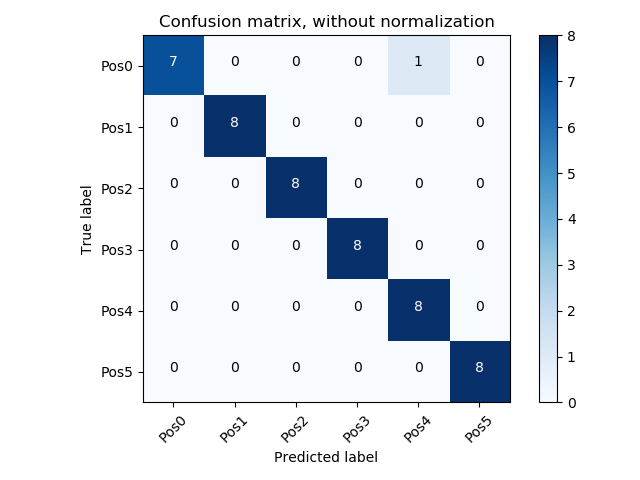
\includegraphics[scale=0.5]{figures/mat_pos_Sx_raw.png}
  \caption{Matrice de confusion obtenue en utilisant les points Sx et les caractéristiques de "ranging"}
  \label{fig:matPosSxTRaw} %% NOTE: always label *after* caption!
 \end{center}
\end{figure}

Afin de valider le système, cinq points supplémentaires par position ont été pris durant une autre période et en ayant probablement une position à peine différente. Il faut préciser que les mesures sur la position 5 ont été effectuées au même moment tant pour les quarante que les cinq mesures. C'est pour cette raison que la détection de cette position est très bonne. 

Cela montre une précision de 46.67\% ce qui correspond à 14 positions correctement reconnues sur 30. Ces résultats ne sont pas encourageants, car cela veut dire que sitôt que l'espion est positionné différemment, mais au même endroit cela influence grandement la reconnaissance. Il est donc nécessaire d'effectuer un travaille supplémentaire pour améliorer cette reconnaissance soit niveau prise de mesure soit niveau du travail sur les caractéristiques. Ce qui a été obtenu dans ce test n'était pas ce qui était attendu au vu des résultats obtenus lors de l'entrainement dans la Figure \ref{fig:matPosSxTRaw}.
%toute les raw
%Accuracy with optimisation 46.666666666666664 %
%Accuracy with optimisation 14 sur 30
%Accuracy 0.4666666666666667
\begin{figure}[htp]
 \begin{center}
  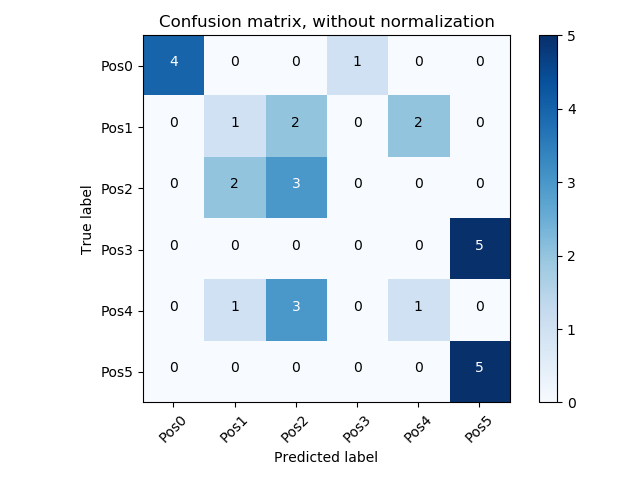
\includegraphics[scale=0.5]{figures/mat_pos_SxT_rawall.png}
  \caption{Matrice de confusion obtenue en utilisant les points de tests SxT et les caractéristiques de "ranging" de la 1ère et 2ème mesures de l'esclave}
  \label{fig:matPosSxTRawall} %% NOTE: always label *after* caption!
 \end{center}
\end{figure}

Deux mesures sont effectuées par esclave pour les quarante canaux. L'exemple précédent prend en compte toutes ces mesures. Afin de voir l'effet de ces mesures, un essai a été de prendre uniquement chaque première mesure et ensuite chaque seconde mesure. Étonnement, cela a amélioré les résultats comme le montre la Figure \ref{fig:matPosSxTRaw1}. Les premières mesures offrent de mauvais résultats alors que prendre uniquement les deuxièmes mesures améliore le score. La précision obtenue est de 53.33\% ce qui correspond à 16 positions correctement reconnues sur 30. Difficile à comprendre pourquoi il y a une amélioration. Afin de clarifier cette influence, il serait intéressant de faire plus de deux mesures par escalve et regarder les différents résultats.
%Accuracy with optimisation 53.333333333333336 %
%Accuracy with optimisation 16 sur 30
%Accuracy 0.5333333333333333
\begin{figure}[htp]
 \begin{center}
  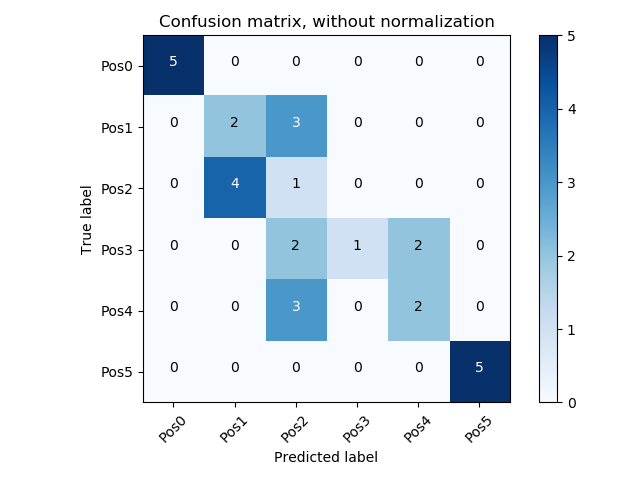
\includegraphics[scale=0.5]{figures/mat_pos_SxT_raw1.png}
  \caption{Matrice de confusion obtenue en utilisant les points de tests SxT et les caractéristiques de "ranging" de la 2ème mesure de l'esclave uniquement}
  \label{fig:matPosSxTRaw1} %% NOTE: always label *after* caption!
 \end{center}
\end{figure}

\subsubsection{Résultat en utilisant la position non convergé}
Le résultat qui est présenté ici permet de faire une comparaison entre une mesure qui est convergée (présenté au chapitre suivant) et une mesure qui est calculée uniquement à partir de huit mesures. C'est sans surprise que les résultats qui sont obtenus sont vraiment moins bons.

La Figure \ref{fig:matPosSxTPos} présente le résultat obtenu lorsque l'entrainement est fait avec 32 des 40 mesures sur une même position et testé avec les huit restants. Le résultat obtenu est impressionnant et offre une précision d'environ 70\% contre environ 85\% pour la solution avec les positions convergées. 

La matrice de confusion représentée est donnée avec des mesures qui ont été faites sur un même point sans bouger l'espion. La précision est de 72.91\%, le F1-score macro est de 0.7102 et un F1-score micro de 0.7293.  
%Accuracy with optimisation 72.91666666666666 %
%Accuracy 0.7291666666666666
%F1-Score macro : 0.7102357609710551
%F1-Score micro: 0.7291666666666665
\begin{figure}[htp]
 \begin{center}
  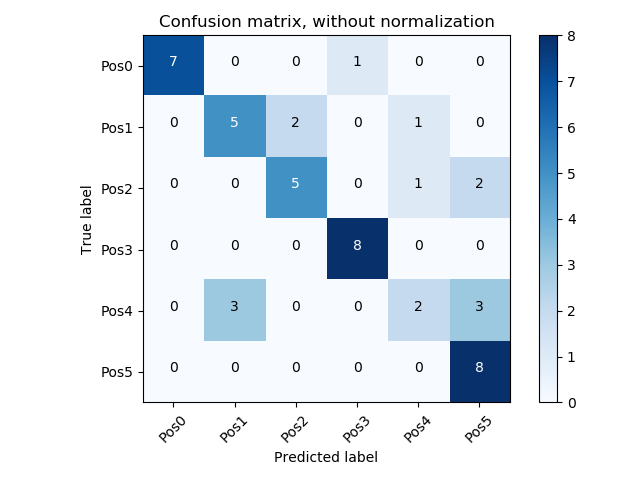
\includegraphics[scale=0.5]{figures/mat_pos_Sx_pos.png}
  \caption{Matrice de confusion obtenue en utilisant les points Sx et la caractéristique de position}
  \label{fig:matPosSxTPos} %% NOTE: always label *after* caption!
 \end{center}
\end{figure}
83.33%

Afin de valider le système, cinq points supplémentaires par position ont été pris durant une autre période et en ayant probablement une position à peine différente. Il faut préciser que les mesures sur la position cinq ont été effectuées au même moment tant pour les quarante que les cinq mesures. C'est pour cette raison que la détection de cette position est très bonne. 

Cela montre une précision de 43.33\% ce qui correspond à 13 positions correctement reconnues sur 30 alors que les résultats pour les positions convergées donnent 83.33\% qui correspond à une reconnaissance correcte de 25 positions sur 30.

%Accuracy with optimisation 43.333333333333336 %
%Accuracy with optimisation 13 sur 30
%Accuracy 0.43333333333333335
\begin{figure}[htp]
 \begin{center}
  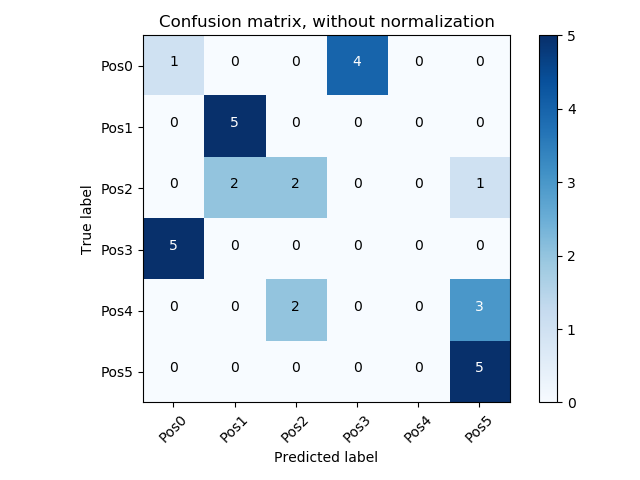
\includegraphics[scale=0.5]{figures/mat_pos_SxT_pos.png}
  \caption{Matrice de confusion obtenue en utilisant les points SxT et la caractéristique de position}
  \label{fig:matPosSxTPos} %% NOTE: always label *after* caption!
 \end{center}
\end{figure}

\subsubsection{Meilleur résultat obtenu}
Ce chapitre va présenter le meilleur résultat qui a été obtenu ainsi que les caractéristiques qui ont été utilisées. Pour y arriver, les caractéristiques suivantes ont été testées de manière individuelle :
 
\begin{enumerate}
 \item Toutes les données "ranging" (raw)
 \item Donnée "ranging" d'un canal (raw) 
 \item La moyenne des canaux
 \item La variance sur les canaux
 \item Déviation standard sur les canaux
 \item Quantile effectué sur les canaux
 \item Médiane effectuée sur les canaux 
 \item Covariance des canaux
\end{enumerate}

Ensuite, plusieurs associations ont été faites entre ses différents tests et le meilleur des résultats est obtenu en associant la valeur de la médiane, de la variance, du quantile et des données de "ranging". À noter que pour avoir le meilleur résultat, il a été nécessaire de prendre en compte uniquement la deuxième mesure de ranging sur chaque esclave. Lorsque les différentes caractéristiques sont affichées, il est à noter que l'amplitude des valeurs n'est pas du même ordre et par conséquent pour tenter de les égaliser, la médiane a été multipliée par cinq, le quantile par six et la variance a été divisée par quatre. Cette façon de faire a encore amélioré les résultats pour obtenir ceux présentés ci-dessous.

La Figure \ref{fig:matPosSx} présente le résultat obtenu lorsque l'entrainement est fait avec 32 des 40 mesures sur une même position et testé avec les huit restants. Cela donne de très bonnes précisions qui se situent entre 83\% et 98\%. Les positions sont majoritairement bien reconnues. La variation de pourcentage pour la reconnaissance vient du fait qu'à chaque lancement, le programme exclut huit autres mesures.

La matrice de confusion représentée est donnée avec des mesures qui ont été faites sur un même point sans bouger l'espion. La précision dans ce cas est de 97.92\% avec un F1-score macro de 0.9791 et un F1-score micro de 0.9792. 

\begin{figure}[htp]
 \begin{center}
  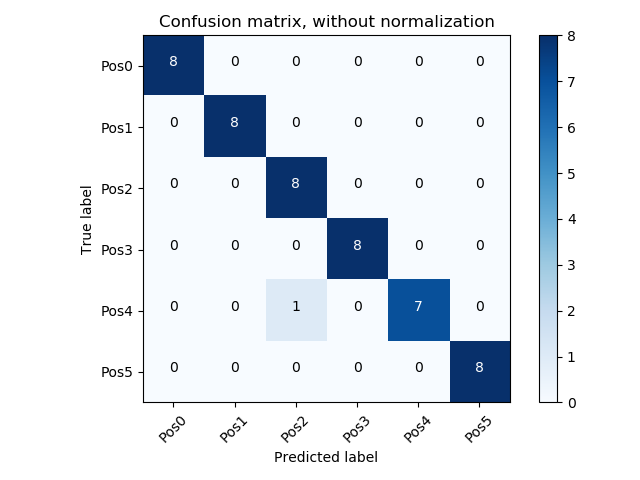
\includegraphics[scale=0.5]{figures/mat_pos_Sx.PNG}
  \caption{Matrice de confusion obtenue pour la meilleure solution en utilisant les données des points Sx}
  \label{fig:matPosSx} %% NOTE: always label *after* caption!
 \end{center}
\end{figure}

Maintenant, afin de valider le système cinq points supplémentaires par position ont été pris durant une autre période de la journée et en ayant probablement une position à peine différente. La présentation des précédents résultats montre de très mauvais résultats concernant ce test, mais après le travail effectué et la recherche des meilleures caractéristiques les résultats sont satisfaisants et encourageants. Il faut préciser que les mesures sur la position 5 ont été effectuées au même moment tant pour les quarante que les cinq mesures. C'est pour cette raison que la détection de cette position est excellente. 

Cela montre une précision de 73.33\% ce qui correspond à 22 positions correctement reconnues sur 30. 
%Accuracy with optimisation 73.33333333333333 %
%Accuracy with optimisation 22 sur 30
%Accuracy 0.7333333333333333
\begin{figure}[htp]
 \begin{center}
  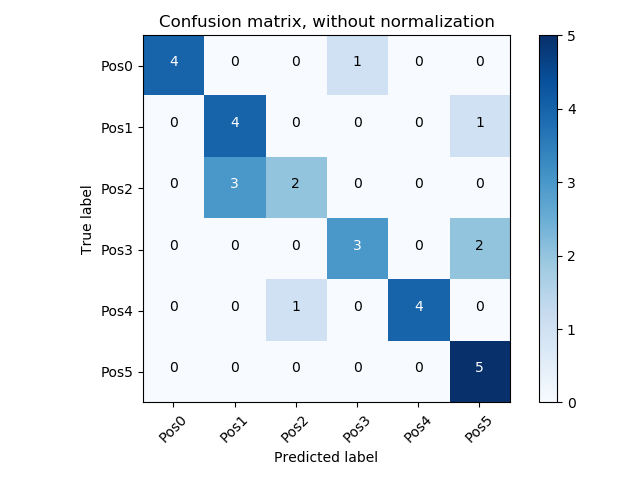
\includegraphics[scale=0.5]{figures/mat_pos_SxT.png}
  \caption{Matrice de confusion pour la meilleure solution en utilisant les points de tests SxT}
  \label{fig:matPosSxT} %% NOTE: always label *after* caption!
 \end{center}
\end{figure}

Un dernier test a été réalisé afin de voir si les positions Tx sont bien reconnues par rapport à leur plus proche voisin. La Figure \ref{fig:matPosTx} montre les résultats obtenus lorsque les positions Tx sont utilisées. Les points T1/2/7/8 correspondent à la position S0, T3/4/9 correspondent à la position S1, T5 correspond à la position S2, T0/6 correspondent à la position S3 et finalement, T10/11/12 correspondent à la position S4. Comme attendu, les résultats pour cette classification ne sont pas bons et pas utilisables. La précision obtenue est de 31.25\% ce qui représente une détection correcte de 20 positions sur 64. Pour obtenir ce résultat, on essaie de classifier les positions Tx selon la position entrainée la plus proche. 

\begin{figure}[htp]
 \begin{center}
  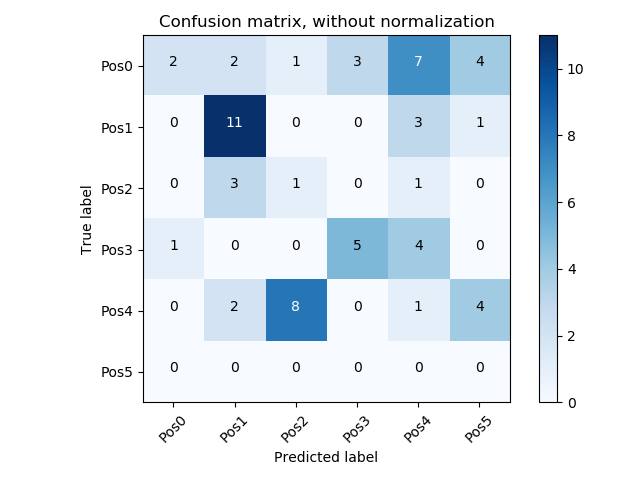
\includegraphics[scale=0.5]{figures/mat_pos_Tx.png}
  \caption{Matrice de confusion pour les valeurs de la position convergée avec des points de tests positionnés autour des points entrainés}
  \label{fig:matPosTx} %% NOTE: always label *after* caption!
 \end{center}
\end{figure}

\subsection{Résultats en utilisant les données de position convergées}
Ce chapitre va présenter les résultats qui ont été obtenus à partir des approximations de position fournies par le programme de mesures. Dans cette partie uniquement ces valeurs seront utilisées. Afin d'avoir une meilleure vue de ce que représentent ces positions, la Figure \ref{fig:plotPosConv} montre le positionnement des points calculés par rapport à la position réelle de l'espion. Les gros points de couleurs représentent la position réelle et les petits points de couleurs représentent les positions calculées. La croix noire représente la position du master. 

\begin{figure}[htp]
 \begin{center}
  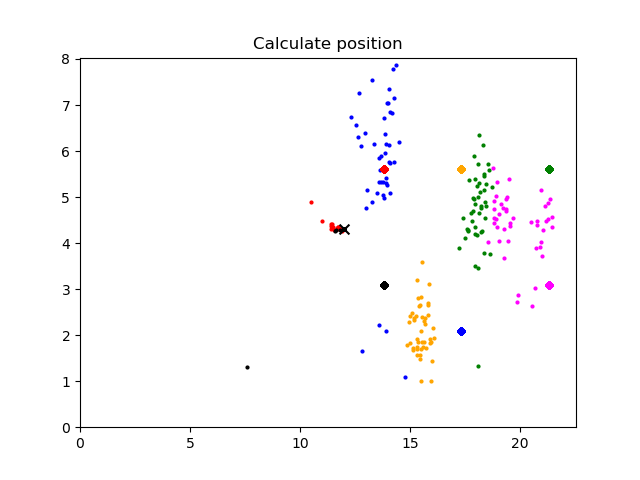
\includegraphics[scale=0.8]{figures/plot_pos_conv.PNG}
  \caption{Représentation des points convergés par rapport aux positions réelles}
  \label{fig:plotPosConv} %% NOTE: always label *after* caption!
 \end{center}
\end{figure}

La Figure \ref{fig:plotPosConv} met en évidence un phénomène qui tend à faire correspondre les points proches du maitre sur les coordonnées du maitre. Cet effet qui se trouve dans le laboratoire où les mesures ont été effectuées complique la reconnaissance de position. De par cette représentation, il est possible de voir à l'oeil nu la séparation des points. Par contre, il est rapidement possible de se rendre compte que si nous ajoutons des points il sera de plus en plus difficile à différencier les emplacements de base de l'espion.

Ci-dessous, une énumération des couleurs et de la position associée : 
\begin{enumerate}
 \item Couleur verte (SO) : x = 21.30m / y = 5.60m
 \item Couleur jaune (S1)  : x = 17.30m / y = 5.60m
 \item Couleur bleue (S2) : x = 17.30m / y = 2.10m
 \item Couleur rose (S3) : x = 21.30m / y = 3.10m
 \item Couleur rouge (S4) : x = 13.80m / y = 5.60m 
 \item Couleur noire (S5) : x = 13.80m / y = 3.10m 
\end{enumerate} 

La Figure \ref{fig:matPosConvSx} représente le résultat obtenu lorsque l'entrainement est fait avec 32 des 40 mesures sur une même position et testé avec les huit restants. Cela donne de très bonnes précisions qui se situent entre 81\% et 89\%. Comme attendu, les positions proches du maitre (S4 et S5) se confondent et pas conséquent ne sont pas correctement reconnues. Les autres positions sont majoritairement bien reconnues à l'exception de quelques mesures. La variation de pourcentage pour la reconnaissance vient du fait qu'à chaque lancement, le programme exclu huit autres mesures.

\begin{figure}[htp]
 \begin{center}
  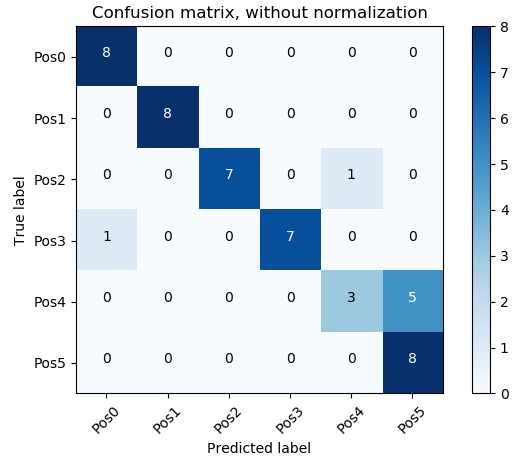
\includegraphics[scale=0.5]{figures/mat_pos_conv_Sx_2.PNG}
  \caption{Matrice de confusion pour les valeurs de la position convergée avec des points positionnés à la même place}
  \label{fig:matPosConvSx} %% NOTE: always label *after* caption!
 \end{center}
\end{figure}

Afin de tester l'algorithme fixé, il est entrainé avec les quarante mesures effectuées sur chaque position de l'espion. Ces quarante mesures sont celles utilisées pour définir les meilleurs paramètres et obtenir les meilleurs résultats comme présentés dans la Figure \ref{fig:plotPosConv}. La Figure \ref{fig:matPosConvSxT} présente le résultat final obtenu avec les cinq données de test qui avaient été effectué à la même position que les quarante de l'entrainement. 

La précision obtenue pour ce test est de 83.33\% ce qui correspond à une reconnaissance correcte de 25 positions sur 30. Les positions mal reconnues sont sans surprise les positions S4 et S5.

\begin{figure}[htp]
 \begin{center}
  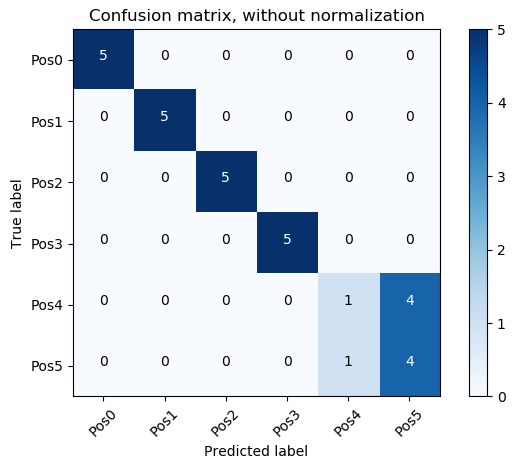
\includegraphics[scale=0.5]{figures/mat_pos_conv_SxT.png}
  \caption{Matrice de confusion pour les valeurs de la position convergée avec des points de tests positionnés à la même place}
  \label{fig:matPosConvSxT} %% NOTE: always label *after* caption!
 \end{center}
\end{figure}

La Figure \ref{fig:matPosConvTx} montre les résultats obtenus lorsque les positions Tx sont utilisées. Les points T1/2/7/8 correspondent à la position S0, T3/4/9 correspondent à la position S1, T5 correspond à la position S2, T0/6 correspondent à la position S3 et finalement, T10/11/12 correspondent à la position S4. Comme attendu, les résultats pour cette classification ne sont pas bons et pas utilisables. La précision obtenue est de 21.67\% ce qui représente une détection correcte de 13 positions sur 60. Pour obtenir ce résultat on essaie de classifier les positions Tx selon la position entrainée la plus proche. 

\begin{figure}[htp]
 \begin{center}
  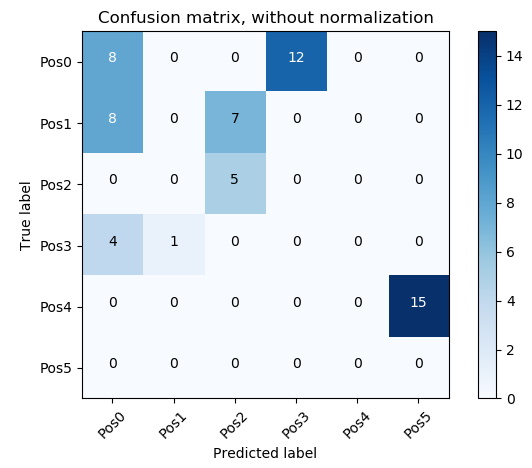
\includegraphics[scale=0.5]{figures/mat_pos_conv_Tx.png}
  \caption{Matrice de confusion pour les valeurs de la position convergée avec des points de tests positionnés autour des points entrainés}
  \label{fig:matPosConvTx} %% NOTE: always label *after* caption!
 \end{center}
\end{figure}

\section{Résumé des résultats}
La Figure \ref{fig:result} résume les résultats présentés dans ce rapport. La solution la plus optimiste a été mise en vert. Ce n'est pas celle qui donne les meilleurs résultats au niveau des points SxT, mais malgré cela c'est elle qui offre la plus grande liberté de traitements et d'améliorations. 

La solution qui utilise uniquement la position convergée donne effectivement de bons résultats, mais si le nombre de points est augmenté ils vont commencer de se mélanger et il ne sera plus possible de les différencier. Les positions proches du maitre seront toujours confondues alors qu'avec la solution d'utiliser les données brutes ces positions sont différenciables. Lorsque les données brutes de "ranging" sont utilisées il est possible d'utiliser des traitements sur ces mesures comme la moyenne, la déviation standard, la variance, etc. chose qui n'est pas possible lorsqu'on possède uniquement l'information des coordonnées x et y. 

\begin{figure}[htp]
 \begin{center}
  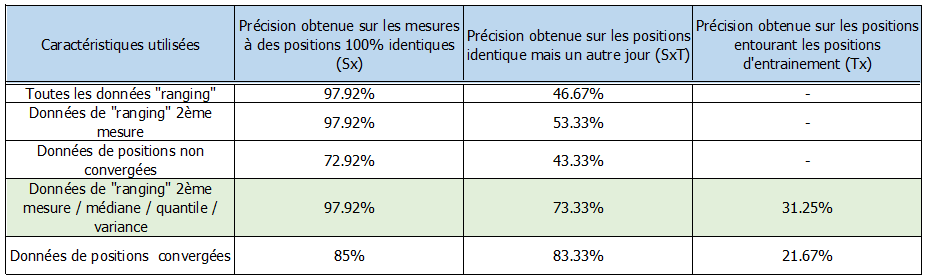
\includegraphics[scale=0.7]{figures/Resultats.png}
  \caption{Résumé des différents résultats obtenus qui sont présentés dans ce rapport}
  \label{fig:result} %% NOTE: always label *after* caption!
 \end{center}
\end{figure}

Un test supplémentaire a été effectué afin de comparer un autre algorithme. Celui utilisé est "random forest", c'est un des algorithmes cité et utilisé dans l'état de l'art. Les résultats obtenus sont inférieurs avec une précision à 50\% ce qui représente une reconnaissance de 15 positions correctes sur 30 contre 22 sur 30 avec l'algorithme SVM. 

\chapter{Problèmes rencontrés et améliorations}
Ce chapitre traite des problèmes qui ont été rencontrés durant de ce travail d'approfondissement ainsi que des améliorations possibles.

Le projet est basé sur une thèse de Master que Michael Mueller avait réalisé \cite{MIC}. Il avait mis en place un programme permettant de calculer une position dans un local intérieur. Réutiliser ce programme devait permettre d'acquérir facilement des mesures, mais cela n'a pas été le cas. Dans un premier temps, il a été nécessaire de modifier le programme, car le système de prise de mesures n'était pas adapté. Cela dans le sens qu'il effectuait des mesures en permanence en stockant les résultats et en recalculant à chaque fois une position par rapport à toutes les mesures. 

Ce qui a été problématique est la stabilité du système qui à tout moment s'arrête de fonctionner et ne donne plus de résultats utilisables. Les esclaves cessaient de fonctionner de temps en temps et cela faisait qu'une mesure prenait un temps conséquent. Il a aussi été remarqué que lorsque le système fonctionnait durant de longues heures d'affilées les bugs étaient de plus en plus nombreux et le système finissait par n'être plus utilisable. 

De plus, lorsque les mesures de positions convergées ont été réalisée afin d'obtenir une série de mesures sur une position (40 mesures sur les 40 canaux), il fallait une demi-journée. Durant ce temps, il faut sans cesse surveiller le système afin de vérifier que les esclaves ne s'éteignent pas. 

Au niveau des améliorations, il serait important de travailler sur le programme de prise de mesures afin de comprendre pourquoi le système s'arrête parfois. Actuellement, la prise est automatique, mais si un des esclaves s'arrête, il faut le redémarrer et cela ne peut pas être fait de manière automatique. 

Un autre point serait de travailler sur un premier tri des mesures afin d'utiliser uniquement celles qui donnent de bons résultats et supprimer les autres (outlier). Cela permettrait d'avoir de meilleurs résultats finaux. Dans le même ordre d'idée, supprimer les canaux qui seraient bruités.

Concernant la compréhension du système complet, faire les mesures dans un environnement maitrisé où les réflexions/absorption sont limitées (ce qui n'est pas le cas dans le laboratoire) serait d'une grande aide. La quantité de mesures prises doit également être augmentée afin de pouvoir poursuivre le travail et se pencher sur une analyse par régression. 

Une réflexion devrait être faite concernant le positionnement des esclaves et du maitre. Il serait éventuellement intéressant d'ajouter un second maitre et de les placer différemment, par exemple aux extrémités plutôt qu'au centre du local. 

Finalement, l'intégration de la mesure du RSSI pourrait être un candidat très intéressant pour compléter l'analyse et améliorer les prédictions. 

%\begin{lstlisting}
% for i=0 to Array.length(t)-1 do
%\end{lstlisting}


%\begin{enumerate}
% \item fgfd
% \item gdgfd
%\end{enumerate}


%\begin{figure}[H]
% \begin{center}
%  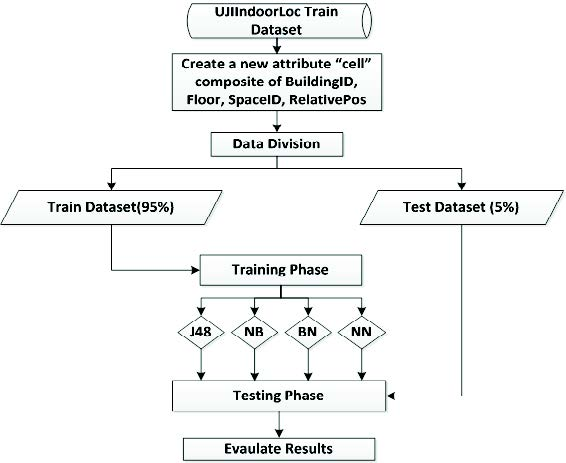
\includegraphics[scale=1]{figures/newattribute.jpg}
%  \caption{The new attribute “cell” construction phase}
%  \label{fig:newAttribute} %% NOTE: always label *after* caption!
% \end{center}
%\end{figure}

%\todo{Compléter cette partie qui semble importante}

